\chapter[Investigation of the VRW-NonRes excess]{Investigation of the $\VRW$-$\NonRes$ excess}
\label{app:ch8_vrw_excess}
\label{subsec:ch8_vrw_excess}

The excess in $\VRW$-$\NonRes$ discussed in Section~\ref{subsec:ch8_vrw} is examined using the cutflow and kinematic distributions.
The pre-fit data and MC simulation yields are consistent through the jet multiplicity requirement, and the discrepancy appears after applying $\met>400~\GeV$, as shown in Figure~\ref{fig:ch8_vrw_cutflow}.
The $N-1$ distribution with finer $\met$ bins in Figure~\ref{fig:ch8_vrw_met_study} shows agreement in most bins, with the excess concentrated in $425<\met<450~\GeV$.
Lowering the $\met$ threshold to $300~\GeV$ or raising it to $500~\GeV$ reduces the discrepancy to $1.8\sigma$ or $1.5\sigma$, respectively, when only statistical uncertainties are considered.

The lepton-$\pT$ distribution within $425<\met<450~\GeV$ is also shown in Figure~\ref{fig:ch8_vrw_met_study}.
The excess is concentrated in $300<\pT^\ell<400~\GeV$, well above the $200~\GeV$ threshold, and is therefore not explained by the lepton-$\pT$ threshold.
The 12 data events in this interval comprise five electron events and seven muon events.
Their lepton and $b$-jet positions are shown in Figure~\ref{fig:ch8_vrw_etaphi}.
The interpretation of these checks is given in Section~\ref{subsec:ch8_vrw}.

% Following figures are from Figs/CH8/studies/; copies without the ATLAS Internal label
% are prepared by scripts/ch8/prepare_vrw_excess_appendix.py.
\begin{figure}[htpb]
    \centering
    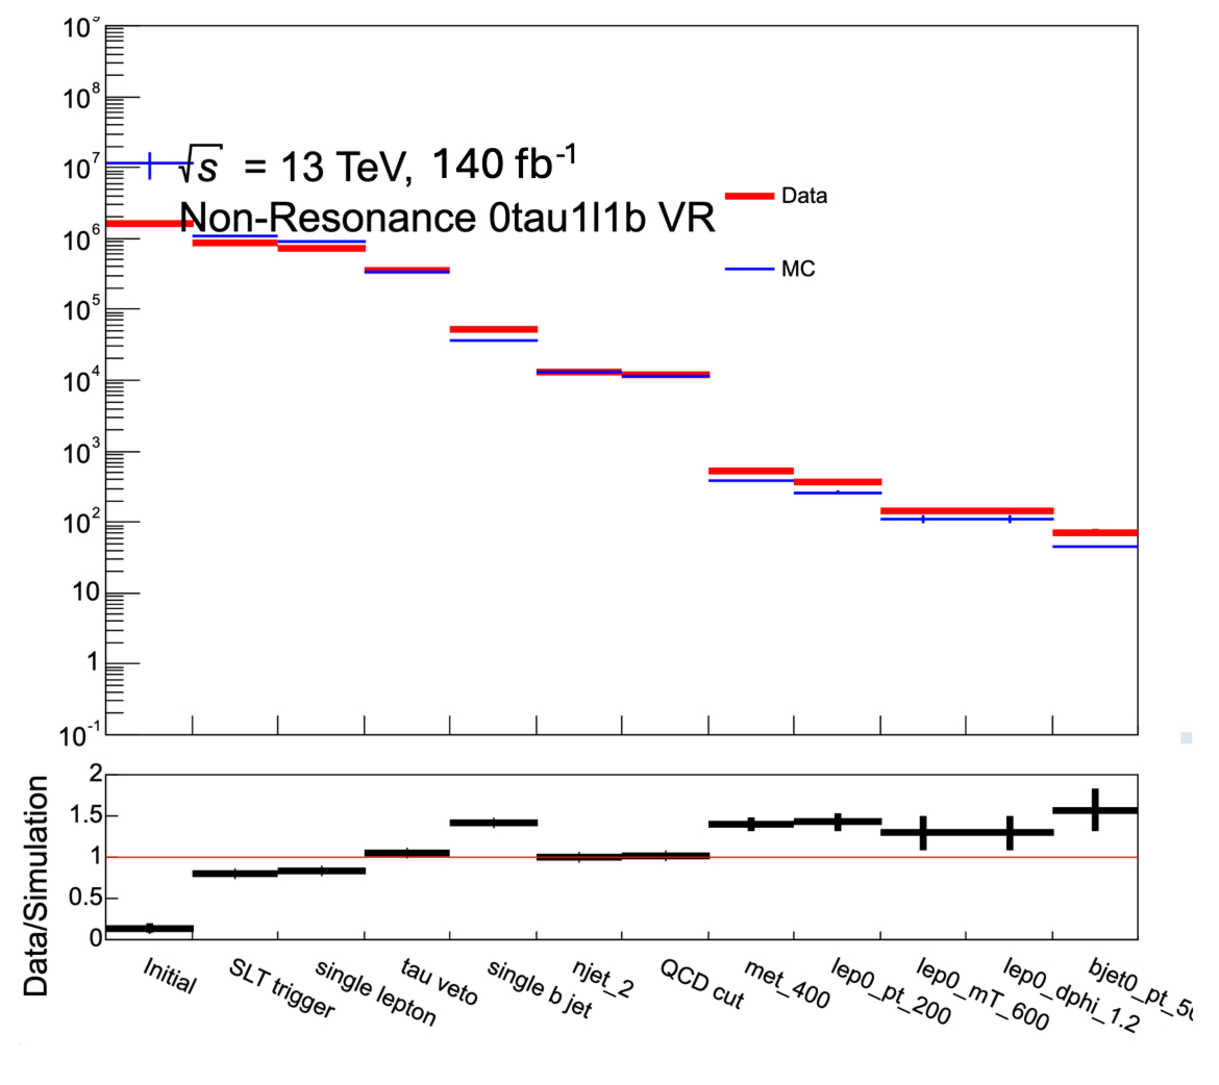
\includegraphics[width=0.86\linewidth]{Figs/CH8/vrw_excess_appendix/VRW_NonRes_cutflow.pdf}
    \caption[Cutflow comparison in VRW-NonRes]{Cutflow comparison between the data and MC for $\VRW$-$\NonRes$.}
    \label{fig:ch8_vrw_cutflow}
\end{figure}

% Following figures are from Figs/CH8/studies/; copies without the ATLAS Internal label
% are prepared by scripts/ch8/prepare_vrw_excess_appendix.py.
\begin{figure}[htpb]
    \centering
    \begin{subfigure}{0.49\linewidth}
        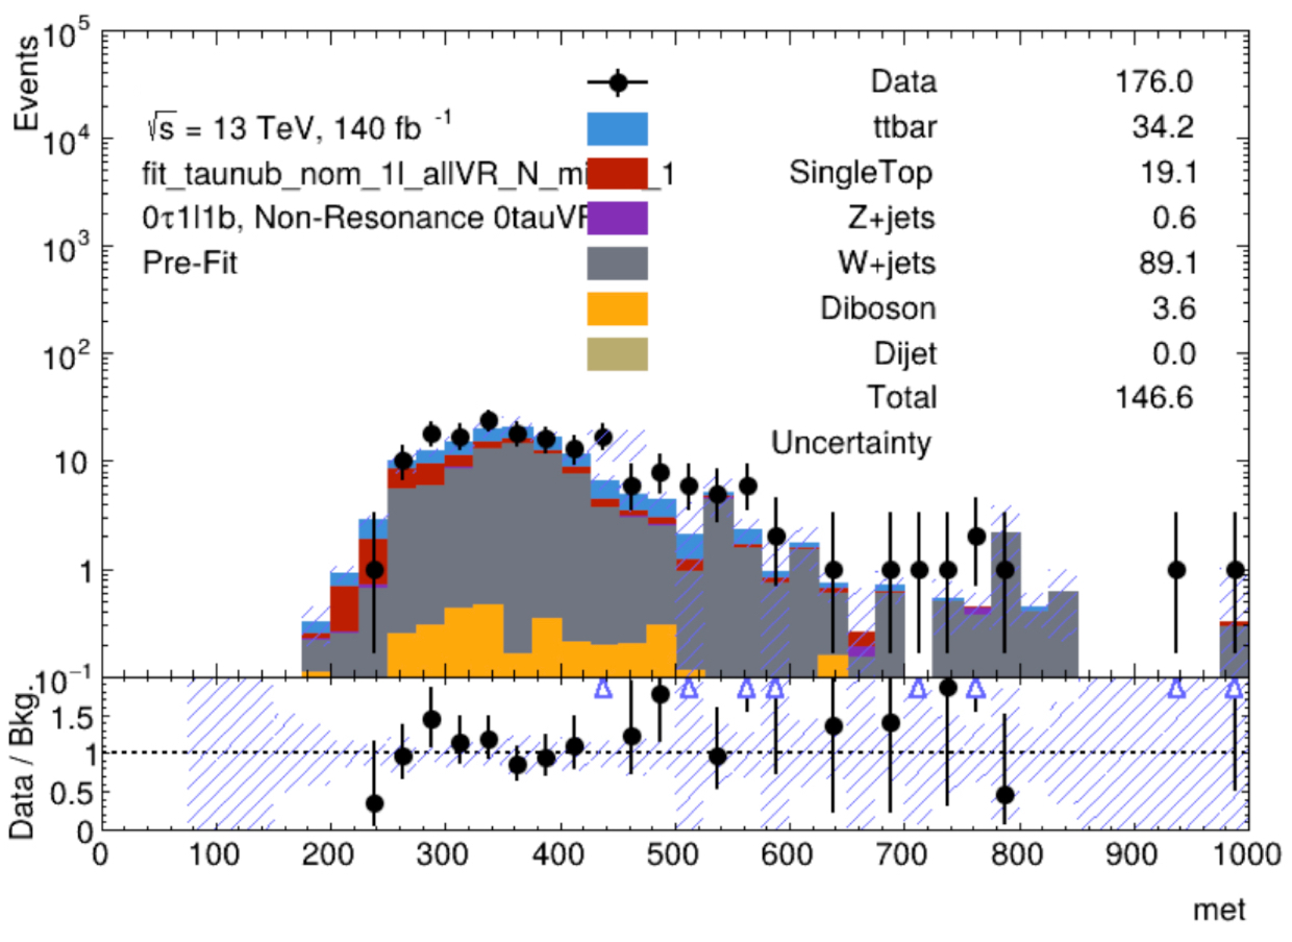
\includegraphics[width=\linewidth]{Figs/CH8/vrw_excess_appendix/VRW_NonRes_fine_met.pdf}
        \caption[]{$\met$ with its threshold removed}
    \end{subfigure}\hfill
    \begin{subfigure}{0.49\linewidth}
        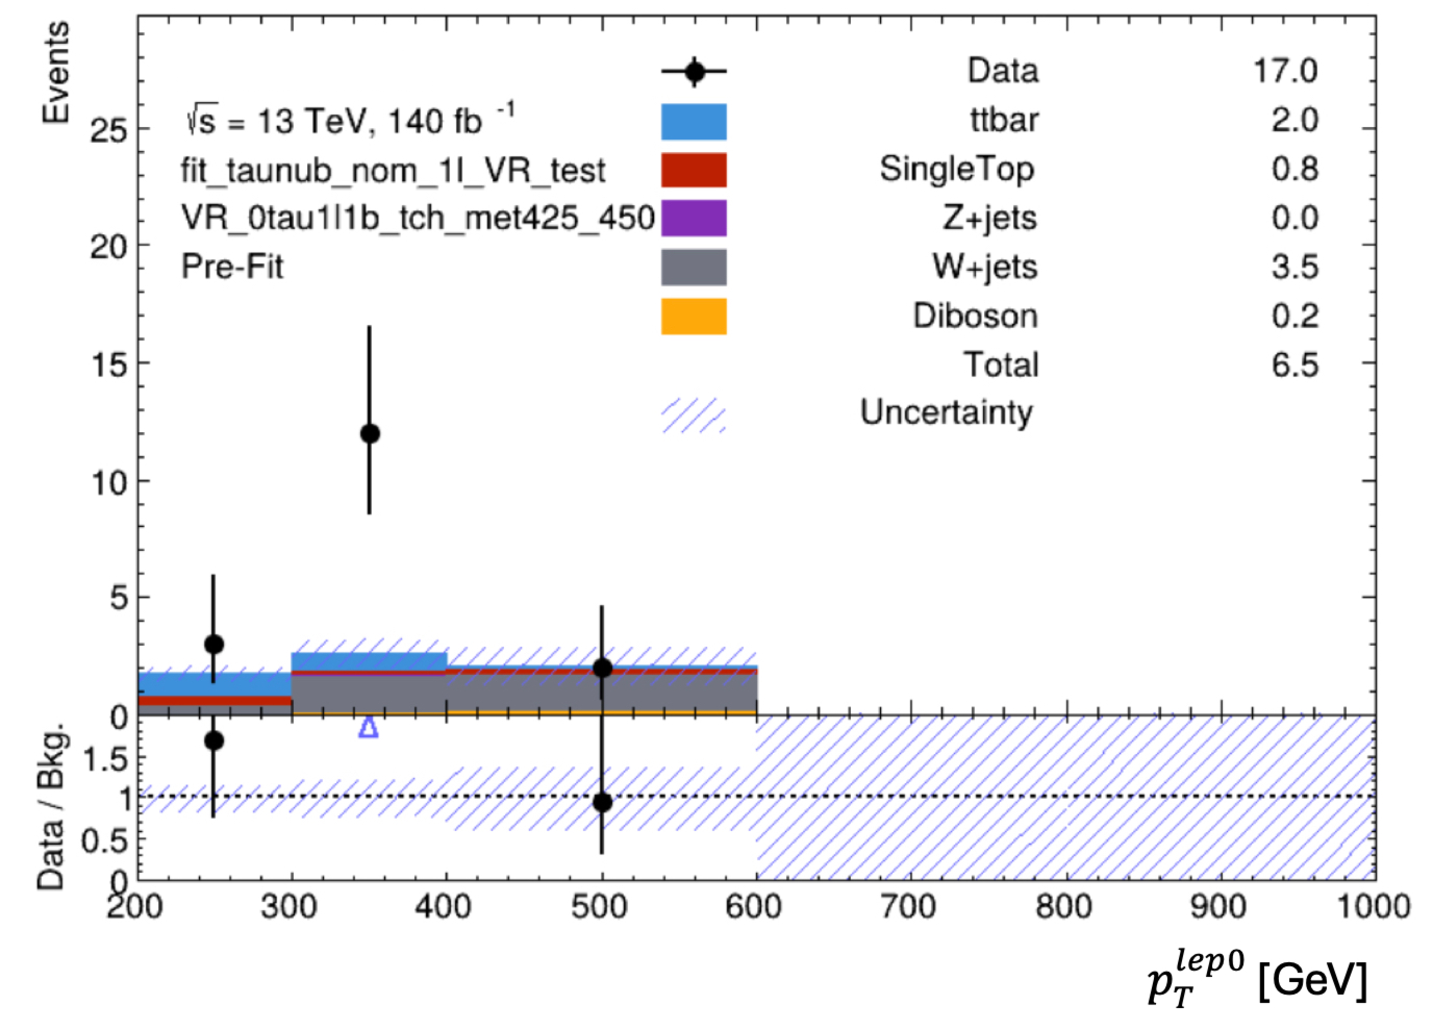
\includegraphics[width=\linewidth]{Figs/CH8/vrw_excess_appendix/VRW_NonRes_local_lep_pt.pdf}
        \caption[]{$\pT^\ell$ for $425<\met<450~\GeV$}
    \end{subfigure}
    \caption[Kinematic localisation of the VRW-NonRes excess]{Left: $N-1$ $\met$ distribution in $\VRW$-$\NonRes$. Data and MC are found to be in rather good agreement for most of the bins. Right: the leading-lepton $\pT$ distribution after applying the $\met$ range cut $425<\met<450~\GeV$, where a large discrepancy between data and the MC expectation is observed.}
    \label{fig:ch8_vrw_met_study}
\end{figure}

% Following figures are from Figs/CH8/studies/; copies without the ATLAS Internal label
% are prepared by scripts/ch8/prepare_vrw_excess_appendix.py.
\begin{figure}[htpb]
    \centering
    \begin{subfigure}{0.49\linewidth}
        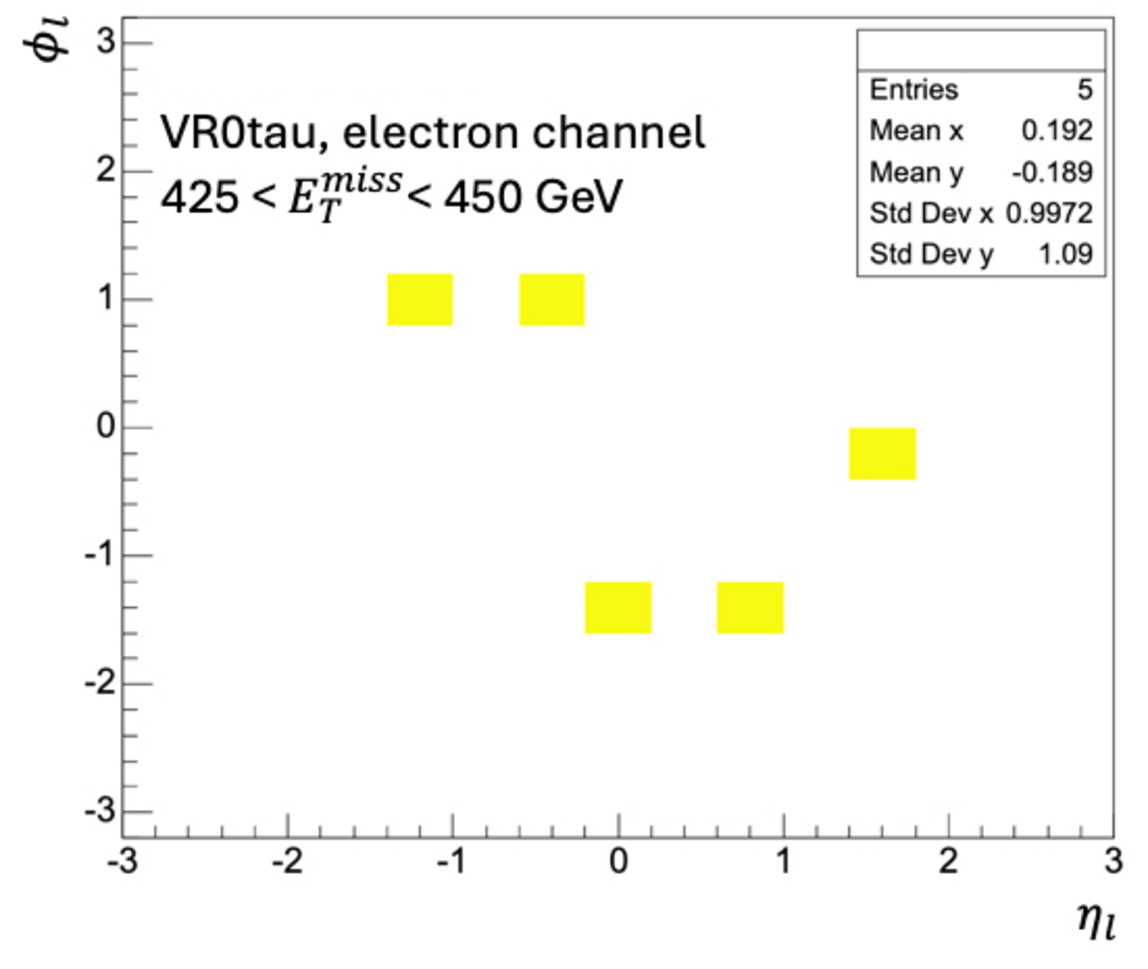
\includegraphics[width=\linewidth]{Figs/CH8/vrw_excess_appendix/VR0tau_echannel_lep_etaphi.pdf}
        \caption[]{Lepton, $e$ channel.}
    \end{subfigure}\hfill
    \begin{subfigure}{0.49\linewidth}
        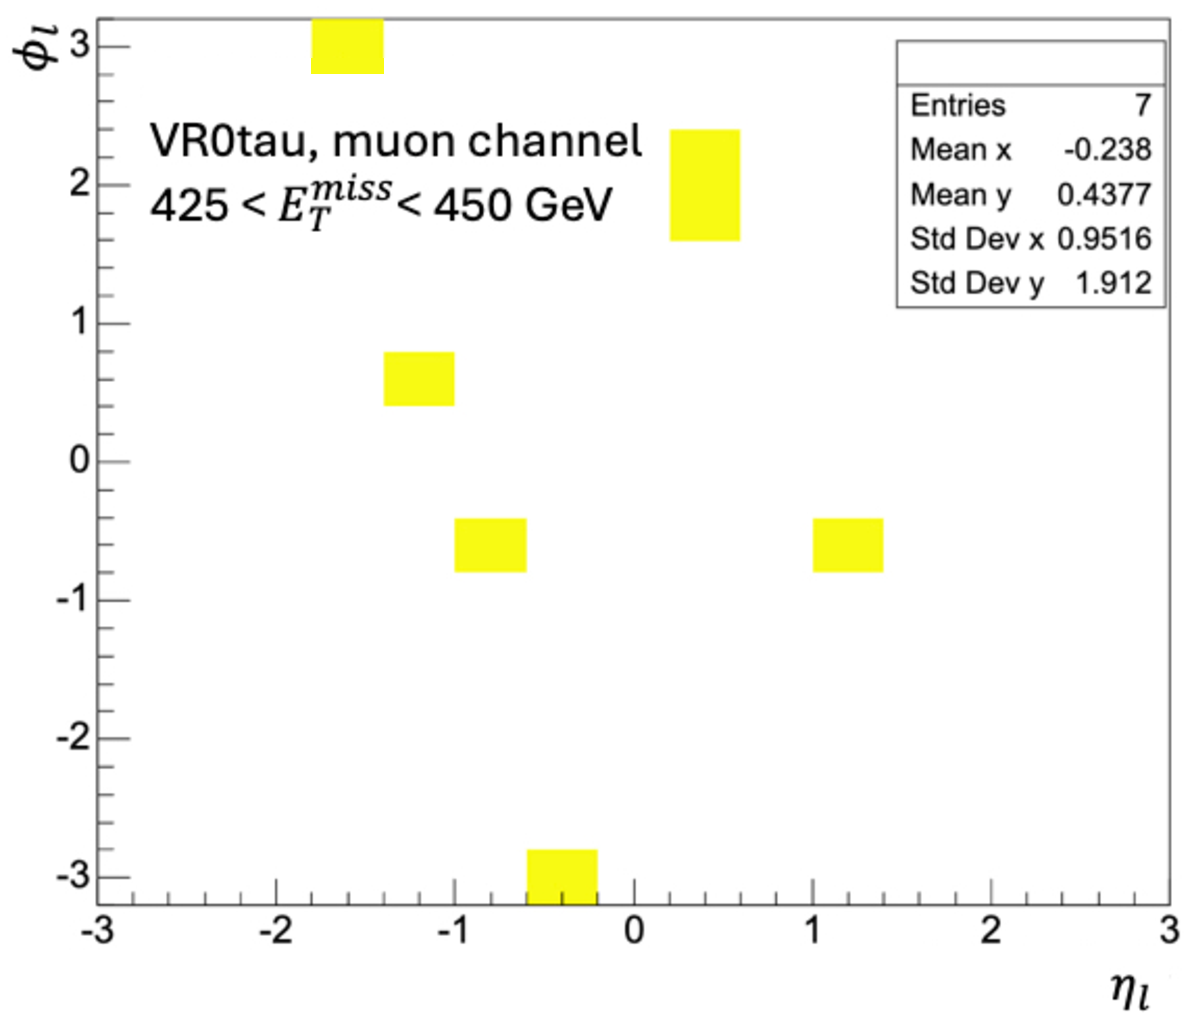
\includegraphics[width=\linewidth]{Figs/CH8/vrw_excess_appendix/VR0tau_muchannel_lep_etaphi.pdf}
        \caption[]{Lepton, $\mu$ channel.}
    \end{subfigure}\\
    \begin{subfigure}{0.49\linewidth}
        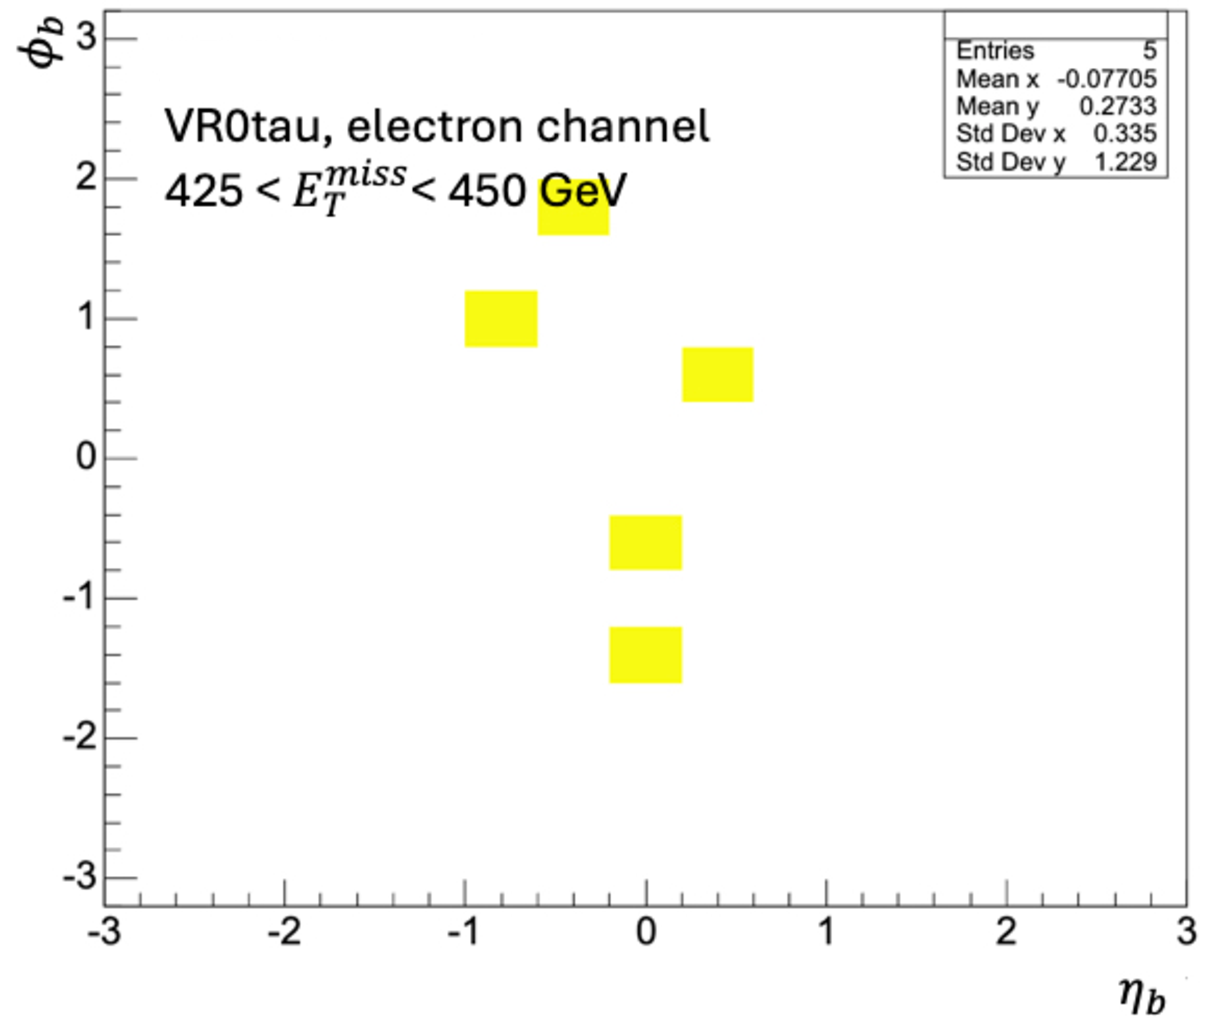
\includegraphics[width=\linewidth]{Figs/CH8/vrw_excess_appendix/VR0tau_echannel_b_etaphi.pdf}
        \caption[]{$b$-jet, $e$ channel.}
    \end{subfigure}\hfill
    \begin{subfigure}{0.49\linewidth}
        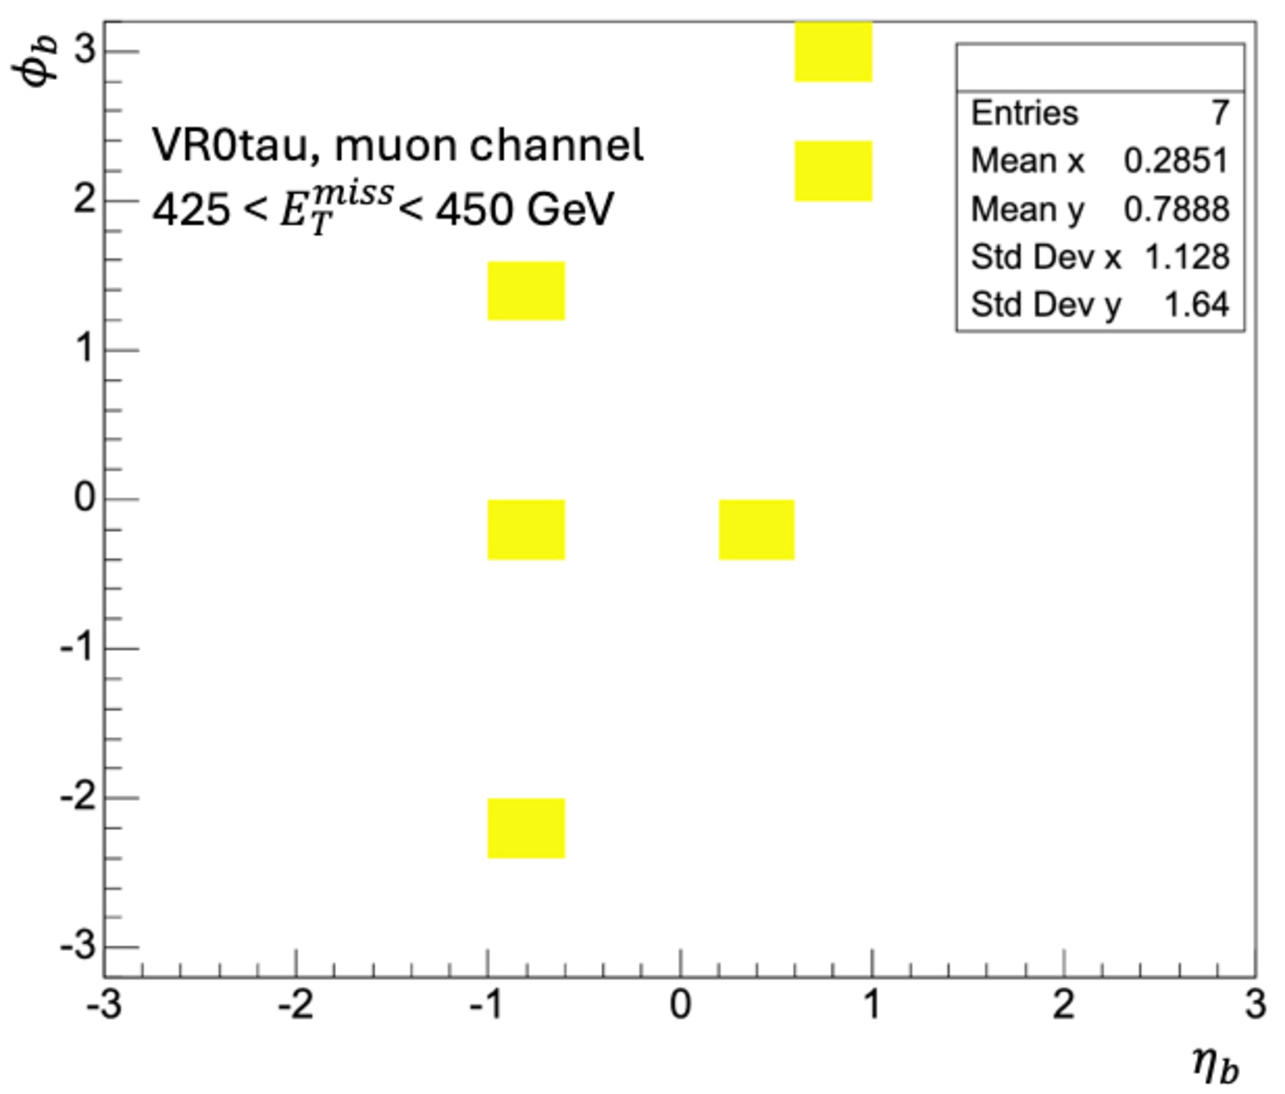
\includegraphics[width=\linewidth]{Figs/CH8/vrw_excess_appendix/VR0tau_muchannel_b_etaphi.pdf}
        \caption[]{$b$-jet, $\mu$ channel.}
    \end{subfigure}
    \caption[Detector positions of events in the VRW-NonRes excess]{$\eta$--$\phi$ map of the lepton and $b$-jets in $\VRW$-$\NonRes$ for the electron channel (left) and the muon channel (right).}
    \label{fig:ch8_vrw_etaphi}
\end{figure}

\clearpage

\section[Low-mass VRs]{Low-mass VRs}
\label{subsec:low_mass_vr}

The low-mass VRs provide the additional $1\hadtau0\ell1b$ check introduced in Section~\ref{sec:ch8_wjets}.
They are used as a supplementary check of the background prediction following the $\VRW$-$\NonRes$ study.

The low-mass VRs are defined by replacing $m_{b\hadtau}>800~\GeV$ with $400<m_{b\hadtau}<800~\GeV$ in the resonant region, and $\mT>600~\GeV$ with $500<\mT<600~\GeV$ in the non-resonant region.
To increase the event yields, the $\mT$ and $\pT^{\hadtau}$ thresholds in the resonant region are both lowered by $100~\GeV$.
In the non-resonant region, the $\met$ threshold is lowered by $200~\GeV$ and the $\pT^{\hadtau}$ threshold by $100~\GeV$.
The resulting selections are summarised in Table~\ref{tab:low_mass_vr}. All other requirements follow the corresponding SR selections.
Signal contamination is checked before examining the data, using the same benchmarks as in the nominal VRs.
It is approximately $2\%$ in the resonant region and $7\%$ in the non-resonant region.

The NFs from a background-only fit to the CRs are then applied to these regions.
This cross-check is performed without systematic uncertainties in the fit.
The predicted and observed yields are given in Table~\ref{tab:low_mass_vr}, and the post-fit comparison is shown in Figure~\ref{fig:ch8_low_mass_vr_summary}.

\begin{table}[htbp]
    \centering
    \small
    \caption[Selections and yields in the low-mass VRs]{Selections and yields in the low-mass VRs. The background-only fit to the CRs is extrapolated to these regions. The systematic uncertainties are not included.}
    \label{tab:low_mass_vr}
    \begin{tabular}{lcc}
        \toprule
         & Resonant & Non-resonant \\
        \midrule
        $\pT^{\hadtau}$ [$\GeV$] & $>100$ & $>100$ \\
        $\met$ [$\GeV$] & $>200$ & $>200$ \\
        $\mT$ [$\GeV$] & $>100$ & $500<\mT<600$ \\
        $m_{b\hadtau}$ [$\GeV$] & $400<m_{b\hadtau}<800$ & No requirement \\
        \midrule
        Signal contamination & $\sim2\%$ & $\sim7\%$ \\
        Post-fit background & $25.4\pm1.5$ & $8.0\pm1.7$ \\
        Observed data & 24 & 9 \\
        \bottomrule
    \end{tabular}
\end{table}

% Following figure is from /Users/zang/Desktop/ICEPP/博士课题/leptoquark/internal_notes/ANA_EXOT_2025_06_INT1/figures/appendix/1tau0l1b_VR_study/Summary_postFit_VR.pdf
% The same diagnostic plot is shown in EB_meeting_260109_v3.pdf, slide 14, and Tau_260115.pdf, slide 7.
% These slides identify the study as a background-only fit without systematics.
% Only ATLAS Internal and the legacy region labels were changed; all 14 bins and both panels are preserved.
% Reproduction and pixel check: output/ch8/vr_restructure_20260925/prepare_lowmass_figure.py and figure_verification.json.
\begin{figure}[htpb]
    \centering
    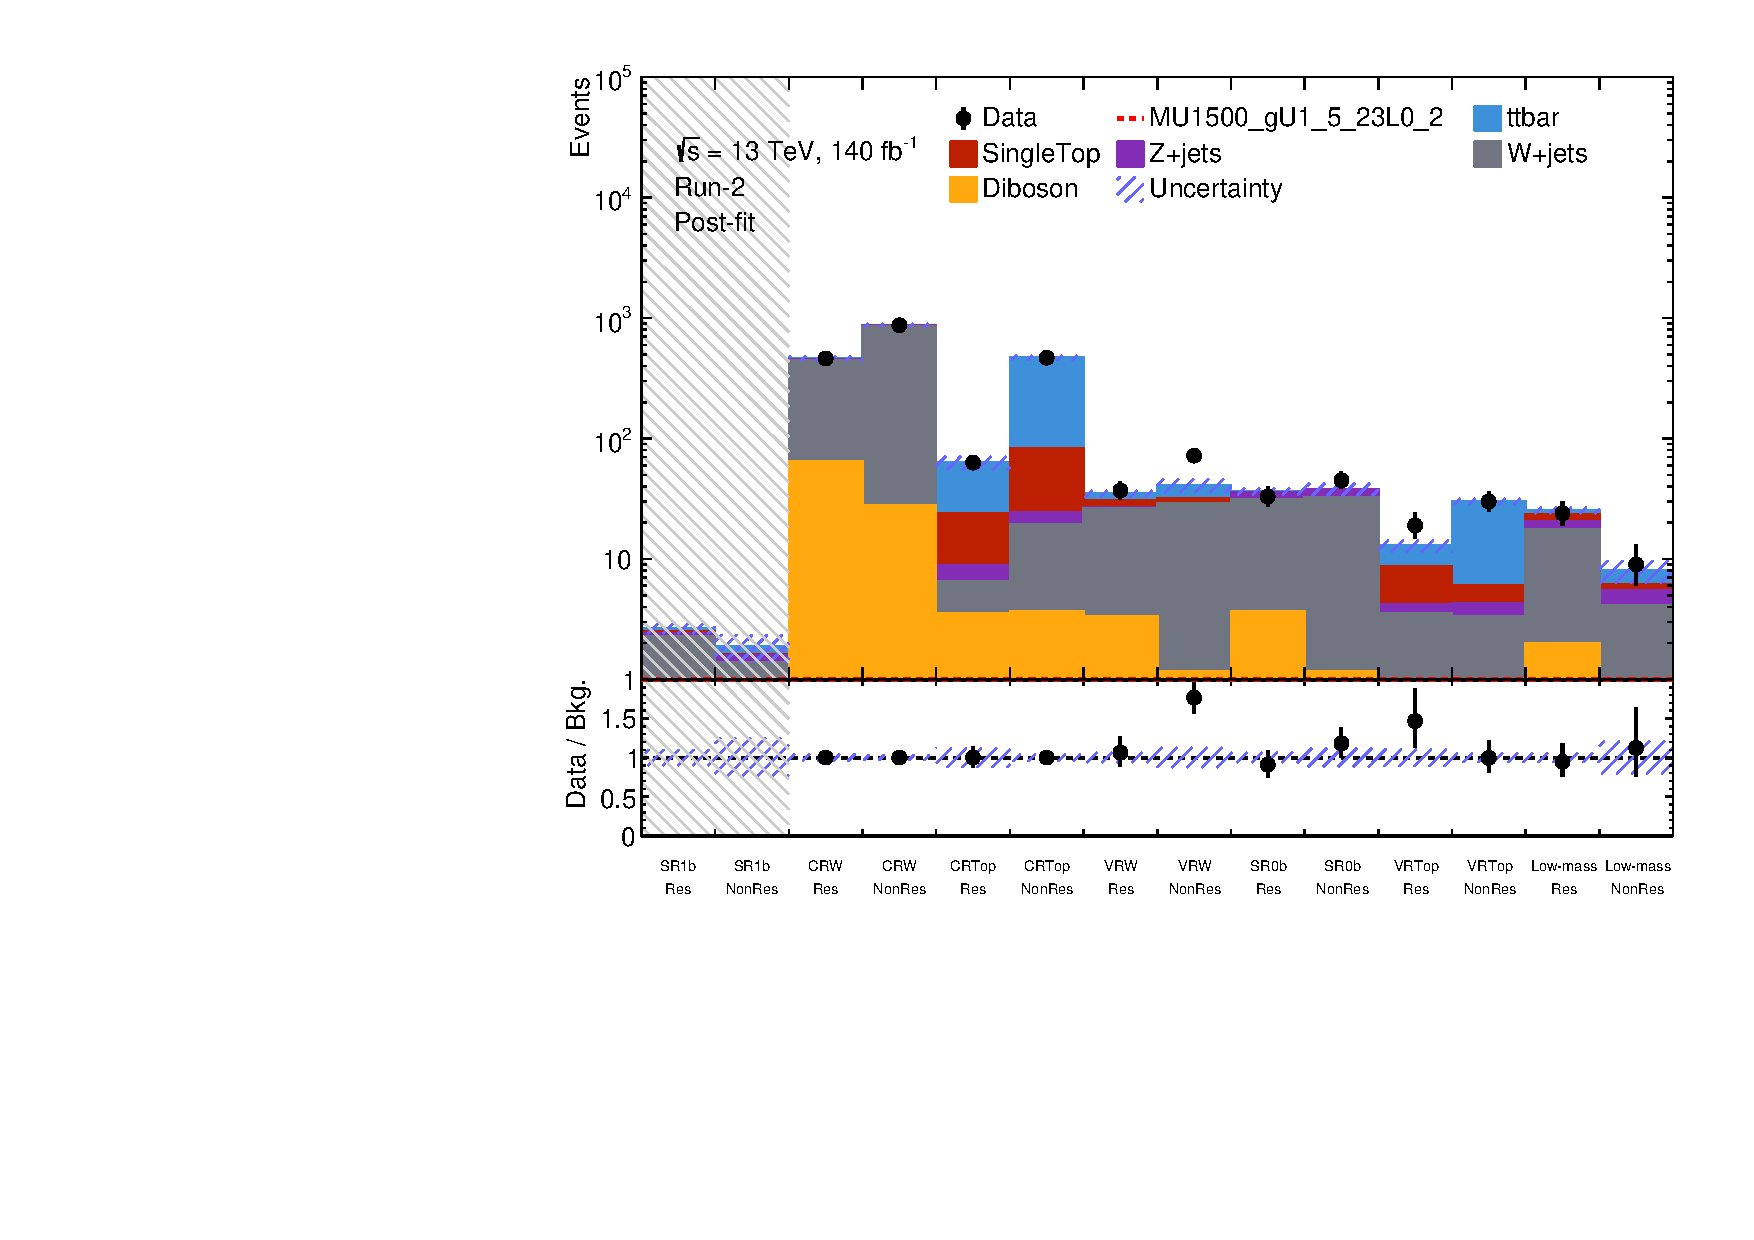
\includegraphics[width=\linewidth]{Figs/CH8/studies/Low_mass_VR_summary.pdf}
    \caption[Background-only fit check in the low-mass VRs]{Post-fit summary plot for the background-only fit without systematic uncertainties. The last two bins stand for the resonant and non-resonant low-mass VRs, respectively.}
    \label{fig:ch8_low_mass_vr_summary}
\end{figure}
